\chapter{PENDAHULUAN}
\titlespacing*{\chapter}{0pt}{0pt}{0pt}
\section{Latar Belakang}
\label{sec:1-LatarBelakang}

\hspace{1,2cm}Televisi merupakan suatu media telekomunikasi satu arah yang menyampaikan informasi dalam bentuk gambar bergerak dan suara. Penerima siaran televisi harus memiliki tv set atau tv receiver, biasa tv set terdiri dari monitor, tuner, speaker, dan antena. Saat ini siaran televisi digital dapat ditransmisikan menggunakan media transmisi radio frekuensi yang biasa kita sebut tv terrestrial, ada juga yang menggunakan kabel, dan juga satelit. Perkembangan teknologi pada bidang penyiaran televisi digital telah menghasilkan beberapa standar diantaranya seperti \textit{Digital Video Broadcasting (DVB), Digital Multimedia Broadcasting (DMB), Integrated Service Digital Broadcasting (ISDB)}, dan \textit{Advanced Television Systems Committee (ATSC)}.  Salah satu standar yang paling banyak digunakan di dunia menurut data dtvstatus adalah DVB \citep{dtvstatus2017}. DVB merupakan standar teknologi untuk pemancar dan penerima siaran televisi digital. DVB digunakan secara luas di seluruh dunia untuk menyiarkan siaran televisi digital melalui saluran udara, kabel, satelit, dan internet. Ada beberapa varian dari standar DVB, termasuk DVB-T untuk siaran udara, DVB-C untuk siaran melalui kabel, DVB-S untuk siaran melalui satelit, dan DVB-I untuk siaran melalui internet \citep{Reimers2006}\citep{Chochliouros2009}.

Pada akhir 2012, Peraturan Menteri Komunikasi dan Informatika Republik Indonesia Nomor 5/PER/M.KOMINFO/2/2012 tentang standar siaran televisi digital terestrial penerimaan tetap tidak berbayar \textit{(Free To Air)}, infrastruktur TV digital menggunakan sistem DVB-T telah dimulai dan dioperasikan oleh penyedia layanan swasta di Jawa dan Kepulauan Riau. Pada periode transisi, sinyal analog dan digital secara bersamaan dipancarkan, yang dikenal sebagai periode \textit{simulcast}. Tujuan periode transisi adalah agar orang-orang mulai membuat transisi ke penyiaran digital dan melihat perbedaan dalam kualitas siaran analog dan digital \citep{Suryanto2021}.

Analog switch off (ASO) adalah proses transisi dari siaran televisi analog ke siaran televisi digital. Di Indonesia, ASO pertama kali dilakukan pada tahun 2018 di wilayah Jakarta, Bandung, dan Surabaya. Proses ASO di Indonesia dilakukan dengan menggunakan teknologi DVB-T2 (Digital Video Broadcasting - Second Generation Terrestrial), yang merupakan versi terbaru dari standar DVB untuk siaran udara. ASO di Indonesia juga dilakukan secara bertahap di beberapa daerah hingga puncaknya tanggal 2 November 2022 \citep{Kominfo2022}. Setelah ASO, siaran televisi analog di Indonesia tidak lagi tersedia dan hanya tersedia siaran televisi digital melalui antena atau parabola satelit. Penggunaan televisi digital diharapkan dapat memberikan kualitas siaran yang lebih baik, serta menambah jumlah saluran yang tersedia. Selain itu, penggunaan teknologi digital juga diharapkan dapat meningkatkan efisiensi penggunaan frekuensi radio dan mengurangi interferensi sinyal \citep{Gultom_2018}. Kelebihan lain dari siaran televisi digital dibanding analog adalah dapat mengurangi dampak dari interferensi sinyal dikarenakan memiliki kemampuan forward error correction  (FEC) untuk memperbaiki data yang rusak \citep{Dai2012}. 

Hingga saat ini siaran televisi baik analog maupun digital merupakan komunikasi satu arah yang memberikan informasi ke pengguna dalam bentuk gambar dan juga suara. Kekurangan dari sistem komunikasi ini adalah pengguna hanya dapat menerima bagaimanapun kualitas dari gambar dan suara yang diterima, tanpa memungkinkan penerima untuk memberikan tanggapan atau berinteraksi dengan pengirim. Seringnya terjadi gangguan pada saluran televisi terutama di daerah-daerah yang jauh dari jangkauan pemancar dapat menimbulkan kerusakan gambar/suara, tidak lengkapnya informasi dan ketidakpuasan pengguna. Hal-hal seperti itu terkadang tidak diketahui oleh penyedia layanan atau stasiun pemancar televisi. Komunikasi satu arah tersebut merupakan karakteristik utama dari televisi, yang membedakannya dengan media komunikasi lain seperti telepon atau internet yang memungkinkan komunikasi dua arah. Namun demikian, beberapa layanan televisi juga dapat menyediakan fitur-fitur interaktif seperti telepon atau pesan teks untuk memungkinkan penerima berinteraksi dengan siaran yang sedang disajikan \citep{HaH.Nguyen2009}. Dikarenakan komunikasi satu arah tersebut, maka kualitas dari siaran dari televisi sering menjadi permasalahan di pengguna yang tidak tersampaikan. Kualitas dari suatu layanan televisi dapat diukur dengan beberapa paramater konvensional seperti tingkat kekuatan sinyal di suatu wilayah, distorsi sinyal dan perbandingan sinyal dengan gangguan (noise ratio). Pengukuran kualitas sinyal, biasanya digunakan alat ukur seperti spetrum analyzer, atau signal level meter.  Alat-alat itu dapat membantu mengukur parameter-parameter tersebut secara akurat dan membantu dalam menentukan keandalan sistem komunikasi. Pengukuran kualitas sinyal sangat penting untuk memastikan bahwa sistem komunikasi dapat berfungsi dengan baik dan memberikan performa yang optimal \citep{GeorgeKennedy2009}.

Parameter pengukuran sinyal sangat penting untuk menentukan kualitas gambar pada siaran televisi digital. Namun, parameter pengukuran sinyal tersebut tidak cukup untuk dapat menggambarkan kualitas dari suatu siaran. Beberapa kasus pada siaran TV digital sering terjadi kerusakan gambar meskipun kekuatan sinyal yang diterima baik. Hal tersebut dikarekan televisi digital menggunakan teknologi kompresi, dan apabila terjadi kerusakan di bagian data yang fatal, maka kerusakan akan lebih parah dibanding pada bagian data lain \citep{Fischer2010}. Pada televisi digital terdapat beberapa jenis kerusakan yang biasa terjadi. Pertama adalah blockiness yaitu dimana gambar yang ditampilkan pada televisi terlihat seperti terdiri dari beberapa blok-blok kecil yang tidak teratur. Kedua yaitu blur dimana gambar yang ditampilkan terlihat kabur atau tidak jelas.  Ketiga yaitu spatial dimana gambar yang ditampilkan tidak teratur atau berhenti. Ketiga parameter kerusakan pada gambar tersebut bisa dijadikan suatu ukuran untuk menentukan kualitas gambar pada siaran televisi digital \citep{MichaelRobin2000}.

Berdasarkan latar belakang masalah yang ada pada siaran televisi digital terrestrial, diperlukan suatu metode untuk dapat melakukan pengukuran kualitas sinyal dan juga kualitas gambar dari sisi penerima. Hasil pengukuran tersebut nantinya dapat menunjukkan seberapa bagus kualitas dari gambar yang diterima dari siaran televisi digital dalam periode tertentu dan juga menggambarkan kepuasan pengguna terhadap siaran yang diterima. Terdapat beberapa jenis pengukuran yang dapat dilakukan untuk mengukur kualitas siaran televisi digital yang pertama yaitu mengukur kualitas sinyal yang diterima dengan menggunakan signal strength meter atau signal quality meter. 

Kedua menggunakan metode digital objective measurement, metode ini menggunakan pengukuran yang dapat memperoleh data kualitas gambar secara objektif, seperti mengukur tingkat kontras, saturasi, kecerahan, resolusi gambar \citep{Wang2003}. Pengukuran kualitas gambar objektif juga dilakukan dengan menggunakan metrik kualitas gambar. Metrik kualitas gambar terdiri dari full-reference (FR), reduced-reference (RR), dan no-reference (NR) \citep{Kusuma2005}. Metrik pengukuran kualitas gambar FR dan RR membutuhkan referensi dari gambar asli untuk melakukan pengukuran. Pada siaran televisi digital metrik FR dan RR tidak dapat digunakan pada pengukuran kualitas gambar tv digital dikarenakan tidak adanya referensi gambar asli yang dapat dibandingan dengan gambar yang diterima dari siaran televisi. Metrik yang dapat digunakan pada pengukuran langsung siaran televisi digital adalah NR metrik seperti no-reference image quality assessment (NR-IQA). 

Pengukuran ketiga menggunakan metode subjective measurement, metode ini menggunakan tes subjektif yang dilakukan oleh responden atau penonton untuk menilai kualitas gambar yang diterima. Metode ini dapat digunakan untuk mengukur kualitas gambar dari sudut pandang penonton. Pengukuran subyektif dapat memakan waktu dan sumber daya yang banyak serta memiliki variasi yang besar dalam hasilnya, tapi dianggap sebagai cara paling akurat untuk mengukur kualitas gambar yang dirasakan. Pengukuran ini juga digunakan sebagai acuan untuk membandingkan pengukuran kualitas obyektif dengan melihat seberapa dekat pengukuran obyektif dapat memprediksi kualitas yang dirasakan oleh manusia. Salah satu metode yang paling sering digunakan adalah Mean Opinion Score (MOS) Metode ini menanyakan pengamat untuk memberikan skor kualitas pada skala 1 sampai 5, dengan skor 5 merupakan kualitas tertinggi dan skor 1 merupakan kualitas terendah. Skor rata-rata dari seluruh pengamat yang memberikan skor digunakan sebagai hasil pengukuran. Terdapat juga beberapa metode lain sepert Single Stimulus (SS) \citep{Romass2013}.

Penelitian ini bertujuan untuk membuat suatu sistem spengukuran secara real-time terhadap kualitas sinyal dan gambar pada siaran televisi digital terrestrial DVB-T2 yang ada di Indonesia. Pengukuran terbagi menjadi dua bagian yang pertama adalah pengukuran sinyal dilakukan menggunakan hardware yang data hasil pengukurannya dapat diakuisisi ke dalam sistem. Kedua pengukuran pada kualitas gambar dilakukan dengan menggabungkan hasil subjective measurement dan objective measurement dalam artifial neural network (ANN). Pengukuran pada penelitian ini difokuskan pada kualitas gambar dari video hasil transmisi DVB-T2, dikarenakan televisi lebih mengutamakan gambar dibanding dengan audio. Evaluasi kualitas video dilakukan untuk menggambarkan kualitas sekumpulan rangkaian video secara real time dalam satuan nominal yang objektif.

 Perangkat yang digunakan adalah microcomputer raspberry-pi dengan tambahan modul perangkat keras untuk memperoleh siaran DVB-T2. Perangkat tersebut digunakan dengan adanya alasan khusus yaitu dari segi ekonomis, dinamis, spesifikasi, dan juga mudah untuk menamakan program. Data hasil pengukuran dengan menggunakan perangkat tersebut nantinya akan dikirimkan menggunakan jaringan internet dengan protocol internet of things (IoT). Hasil dari sistem ini adalah suatu aplikasi website yang menunjukkan grafik pengukuran sinyal dan juga grafik pengukuran kualitas gambar menggunakan algoritma ANN yang disesuaikan dengan standar pengukuran ITU-R BT.500-14 yang dirilis tahun 2019. Penelitian mengenai sistem pengukuruan kualitas gambar pada siaran televisi digital menggunakan machine learning masih sangat jarang ditemukan sehingga menjadi suatu peluang penelitian dan pengembangan.
 

\section{Rumusan Masalah}
\label{sec:2-Rumusanmasalah}
\hspace{1,2cm}Berdasarkan pada topik penelitian yang telah uraikan pada latar belakang di atas, maka diperoleh beberapa rumusan masalah yang menjadi fokus pada penelitian, yaitu:
\begin{enumerate}
 \item Bagaimana cara melakukan akuisi data pengukuran kualitas siaran televisi digital menggunakan perangkat komputer?
 \item Bagaimana menerapkan algoritma pengukuran NR-IQA yang ada pada perangkat computer untuk melakukan pengukuran objektif kualitas gambar ?
 \item Bagaimana cara untuk melakukan pengukuran subjektif terhadap gambar/video dari siaran televisi digital terrestrial? 
 \item Bagaimana menerapkan model ANN berdasarkan pengukuran objektif dan subjektif pada pengukuran kualitas gambar siaran televisi digital terrestrial secara real-time?   
\end{enumerate}

\section{Batasan Masalah}
\label{sec:3-BatasanMasalah}
\hspace{1,2cm}Penelitian ini berusaha mengembangkan teknik dan mengatasi kendala yang telah ada dalam bentuk pembuatan sistem untuk melakukan pengukuran kualitas sinyal dan kualitas gambar dari siaran televisi digital terrestrial secara real-time sehingga Batasan pada penelitian ini yaitu:
\begin{enumerate}
	\item Menggunakan perangkat mikrokomputer raspberry-pi dan modul tv hat untuk mendapatkan siaran televisi digital terrestrial (DVB-T2) dan juga pengukuran kualitas sinyal yang dapat diakuisisi pada perangkat komputer. Perangkat ini memiliki kekurangan dari sisi spesifikasi prosesor dan juga GPU yang tidak terlalu tinggi. 
	\item Menggunakan beberapa pengukuran no-reference image quality metrics (NR-IQA) yang sudah ada untuk mendapatkan tingkat kerusakan pada gambar secara objektif yang nantinya digunakan sebagai variable masukan pada sistem artificial neural network (ANN).
	\item Melakukan pengukuran secara subjektif pada gambar/video menggunakan standar terbaru yang ditetapkan International Telecommunication Union (ITU). Hasil pengukuran ini nantinya digunakan sebagai parameter supervised learning pada sistem ANN.
	\item Melakukan implementasi model dari ANN ke sistem untuk melakukan pengukuran secara realtime pada mikrokomputer. Hasil pengukuran dikirim menggunakan protocol IoT yang nantinya ditampilkan pada aplikasi web.
\end{enumerate}

\section{Tujuan Penelitian}
\label{sec:4-TujuanPenelitian}
\hspace{1,2cm}Berdasarkan masalah penelitian yang telah diuraikan sebelumnya, maka tujuan utama dari penelitian ini adalah membuat suatu sistem pengukuran kualitas sinyal dan kualitas gambar pada siaran televisi digital terrestrial. Dalam prosesnya dibutuhkan beberapa tujuan yang ingin dicapai dalam penelitian ini, yaitu:
\begin{enumerate}
	\item Menghasilkan metode untuk memeperoleh data kualitas sinyal televisi digital terrestrial secara realtime menggukan perangkat mikrokomputer.
	\item Menghasilkan suatu model ANN dengan variable masukan berupa pengukuran objektif kualitas gambar yang disupervised menggunakan pengukuran subjektif.
	\item Membuat suatu aplikasi untuk melakukan pengukuran gambar/video dari siaran televisi digital secara subjektif, yang nantinya digunakan sebagai dataset pada ANN. 
	\item Menghasilkan suatu metode untuk melakukan pengukuran kualitas gambar/video secara realtime dari siaran televisi digital menggunakan model ANN yang sudah dibentuk, dan menampilkannya pada dashboard web aplikasi menggunakan protocol IoT. 
\end{enumerate}

\section{Kontribusi dan Manfaat Penelitian}
\label{sec:5-KontribusidanManfaatPenelitian}
\hspace{1,2cm}Dari segi keilmuan, penelitian ini menghasilkan suatu metode untuk melakukan pengukuran kualitas gambar/video menggunakan algoritma ANN supervised learning berdasarkan penilaian subjektif assessment dan juga metrik pengukuran objektif. Dari sisi pengembangan teknologi, penelitian ini menghasilkan suatu sistem pengukuran kualitas gambar/video pada siaran televisi digital terrestrial secara realtime. Sistem ini dapat digunakan secara umum untuk mengetahui kualitas siaran televisi pada suatu wilayah.

Manfaat dari penelitian ini yaitu sistem yang dihasilkan dapat diterapkan dan digunakan oleh penyedia siaran (services), pengguna jasa siaran, dan juga pengguna akhir. Sistem dapat menampilan secara realtime dengan pengukuran yang sesuai untuk dapat memeberikan bukti secara nyata kualitas gambar yang diterima di suatu wilayah.

%%%%%%%%%%%%%%%%%%%%%%%%%%% GAMBAR %%%%%%%%%%%%%%%%%%%%%%%%%%%%%%
%\begin{figure}[!h]
%  \vspace{-0.1cm}
%%\rule{\columnwidth}{0.1pt}
%\begin{center}
%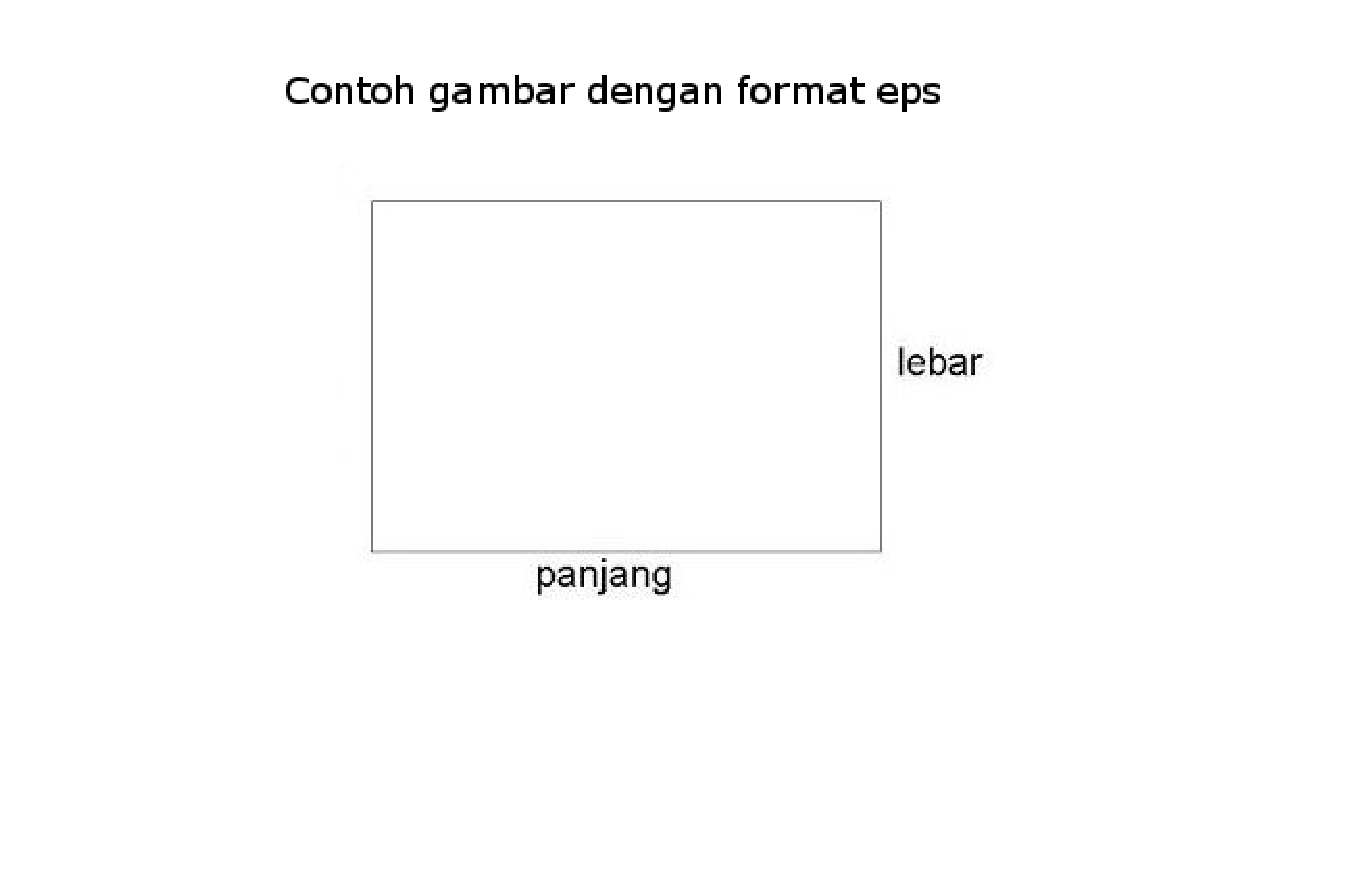
\includegraphics[width=0.8\columnwidth]{bab1/Gambar/gambar1-1.eps}
%\end{center}
%\vspace{-0.2cm}
%%\rule{\columnwidth}{0.1pt}
%\caption{Perbedaan Alur Desain FPGA dan Desain ASIC}\label{gambar1}
%\end{figure}
%%%%%%%%%%%%%%%%%%%%%%%%%%% GAMBAR %%%%%%%%%%%%%%%%%%%%%%%%%%%%%%

